% !TeX spellcheck = en_US 
\documentclass[]{article}
\usepackage[paper=a4paper, left=2.5cm, right=2.5cm, top=2.5cm, bottom=2.5cm]{geometry}
\usepackage[section]{placeins}
\usepackage[indent=0cm]{parskip}
\usepackage[colorlinks, linkcolor=blue, urlcolor=magenta, citecolor=teal, bookmarks]{hyperref}

\usepackage{pack}

\title{
  {\Huge Notebook on the \textit{Colloquio}} \\
  \colloquioTitle
}

\author{
  \myFullName \\
  {\small Advisor: \advisorFullName}
}

\begin{document}
  \maketitle
  \begin{abstract}
    I'm writing this document for my personal use. It's a collection of notions,
    definitions, reflections, and more, produced as I worked on the \textit{colloquio}.
    I hope that this will help me during the preparation of the talk!
  \end{abstract}
  \tableofcontents
  \clearpage
  
  \part{Theoretical foundation}
  \section{The model}
  Restricted Boltzmann Machines are a model used mainly for unsupervised learning. We collect
  data from an unknown distribution and then use it to set the parameters of the RBM to match
  the starting distribution as closely as possible.
  
  \subsection{General RBM}
  Consider a fully-connected bipartite undirected graph as shown in Figure~\ref{fig:generalRBM}.
  It consists of \emph{visible} layer with $m$ nodes labeled by \(V_1, \dots, V_m\) and a
  \emph{hidden} layer whose \(n\) nodes are labeled by \(H_1, \dots, H_n\). We call \(\mathcal{V}\)
  the set of visible nodes, and \(\mathcal{H}\) the set of hidden nodes.
  \begin{figure}
    \centering
    \resizebox{0.5\textwidth}{!}{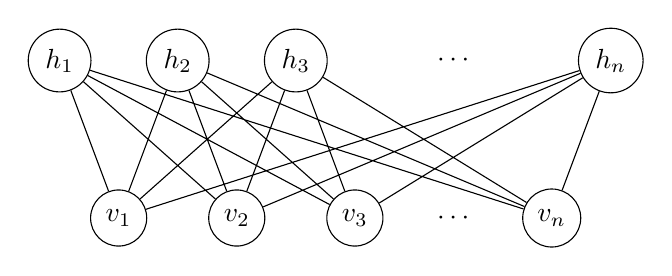
\begin{tikzpicture}%[node distance={15mm}, thick, main/.style = {draw, circle}] 
  \node[draw, circle] (h1) at (1.5,1)   {$h_1$}; 
  \node[draw, circle] (h2) at (3,1)   {$h_2$};
  \node[draw, circle] (h3) at (4.5,1)   {$h_3$};
  \node            (hdots) at (6.5,1) {$\cdots$};
  \node[draw, circle] (hn) at (8.5,1)   {$h_n$};
  
  \node[draw, circle] (v1) at (2.25,-1)   {$v_1$}; 
  \node[draw, circle] (v2) at (3.75,-1)   {$v_2$};
  \node[draw, circle] (v3) at (5.25,-1)   {$v_3$};
  \node            (vdots) at (6.5,-1) {$\cdots$};
  \node[draw, circle] (vm) at (7.75,-1)   {$v_n$};
  
  \draw (v1)--(h1)
        (v1)--(h2)
        (v1)--(h3)
        (v1)--(hn)
        (v2)--(h1)
        (v2)--(h2)
        (v2)--(h3)
        (v2)--(hn)
        (v3)--(h1)
        (v3)--(h2)
        (v3)--(h3)
        (v3)--(hn)
        (vm)--(h1)
        (vm)--(h2)
        (vm)--(h3)
        (vm)--(hn);
\end{tikzpicture} }
    \caption{An RBM graph with \(n\) hidden and \(m\) visible nodes.}
    \label{fig:generalRBM}
  \end{figure}
  Let us consider a random variable \(X_U\) associated with a node \(U\) (either visible or hidden)
  that takes values in \(\Lambda_U\). We say that our graph satisfies the \emph{Markov
  property} if 
  \begin{align*}
    \CondProb{X_v}{\{X_{v'}\}_{v'\in (\mathcal{V} \setminus \{v\})}, \{X_h\}_{h\in \mathcal{H}}} =
    \CondProb{X_v}{\{X_h\}_{h\in \mathcal{H}}}, \\
    \CondProb{X_h}{\{X_v\}_{v\in \mathcal{V}}, \{X_{h'}\}_{h'\in (\mathcal{H} \setminus \{h\})}} =
    \CondProb{X_h}{\{X_v\}_{v\in \mathcal{V}}}.
  \end{align*}
  or saying it simpler: a visible node is independent of all other visible nodes,
  and the same for hidden ones. The graph structure is telling us the dependencies between
  the random variables: if 2 nodes are not connected their associated variables are independent.
  We will assume that \(\Lambda_v = \Lambda_{v'} \,\, \forall v,v' \in \mathcal{V}\) and analog
  for the hidden variables. For simplicity we use the notation
  \[\prob{\vec{v}, \vec{h}} = \Prob{X_{V_i} = v_i, X_{H_j} = h_j
                                    \quad\forall i \in \{1,\dots,m\}, \forall j \in \{1,\dots,n\}}.\]
  
  
  It follows from \emph{Hammersley-Clifford Theorem}\cite{fischer2012introduction} that 
  \begin{equation} \label{eq:hammersley-clifford-thm}
    \prob{\vec{v}, \vec{h}} = \frac{1}{Z} \prod_{i=1,j=1}^{m,n} \psi_{i,j}(v_i, h_j),
  \end{equation}
  where
  \[Z = \sum_{\vec{v}, \vec{h}}\prod_{i=1,j=1}^{m,n} \psi_{i,j}(v_i, h_j)\]
  is called \emph{partition function} and \(\psi_{i,j}\) are called \emph{potential functions}.
  The equation~\eqref{eq:hammersley-clifford-thm} can be written in a more convenient way as
  \begin{equation} \label{eq:RBMdistribution}
    \prob{\vec{v}, \vec{h}} 
      = \frac{1}{Z} \exp\left(\sum_{i=1,j=1}^{m,n}\log\left(\psi_{i,j}(v_i, h_j)\right)\right)
      = \frac{1}{Z} \exp\left(-E(\vec{v}, \vec{h})\right)
  \end{equation}
  where \(E(\vec{v}, \vec{h})=-\sum_{i=1,j=1}^{m,n}\log\left(\psi_{i,j}(v_i, h_j)\right)\) is called
  \emph{energy function}. It should be clear the link with statistical mechanics since equation~\eqref{eq:RBMdistribution}
  is a \emph{Boltzmann distribution} where \(\beta\) (inverse of the temperature) is set to 1. 
  We can go further with the physical interpretation observing that there could be ``interaction''
  only between nodes of different layers, so only when nodes are directly connected: the graph
  structure is again useful to understand RBMs.
  
  The division between visible and hidden nodes is used because only the visible one represents the
  features of the goal distribution; the hidden nodes can be thought of as hidden features that
  the model learns during training. Given this context, it's particularly important the marginal
  distribution
  \[\prob{\vec{v}} = \sum_{\vec{h}} \prob{\vec{v},\vec{h}}.\]
  The Markov property above easily imply this relations on conditional probabilities
  \[
    \condprob{\vec{h}}{\vec{v}} = \prod_{j=1}^n \condprob{h_j}{\vec{v}} \quad\text{and}\quad
    \condprob{\vec{v}}{\vec{h}} = \prod_{i=1}^m \condprob{v_i}{\vec{h}}.
  \]
  
  We empathize that the energy function must be sum of functions of at most 2 nodes;
  the most general energy for an RBM is
  \begin{equation} \label{eq:energyRBM}
    E(\vec{v}, \vec{h}) = \sum_{i}^m f_i{(v_i)} + \sum_{j}^n g_j{(h_j)} +
                          \sum_{i=1,j=1}^{m,n} I_{i,j}{(v_i,h_j)}
  \end{equation}
  
  \subsubsection{Maximum Likelihood}
  We suppose that the energy depends on a set of parameters \(\vec{\theta}\), so it is the function
  \(E(\vec{v}, \vec{h};\vec{\theta})\); obviously also all the other objects of the RBM depend on these parameters. The standard way of estimating parameters in a statistical
  model is maximizing the likelihood. Suppose that our \emph{training set} is 
  \(S = \left\{\vec{\bar{v}}_k\right\}_{k \in \{1,\dots,\ell\}}\) so that the likelihood
  \begin{align*}
    \log\likelihood{\vec{\theta}}{S}
      &= \sum_{k=1}^\ell \log\left(\prob{\vec{\bar{v}}_k;\vec{\theta}}\right)
       = \sum_{k=1}^\ell \log\left(\sum_{\vec{h}} 
                                      \exp\left[-E(\vec{\bar{v}}_k,\vec{h};\vec{\theta})\right]\right)
         -\ell \log{Z(\vec{\theta})} \\
      &= \sum_{k=1}^\ell \log\left(\sum_{\vec{h}} 
                                      \exp\left[-E(\vec{\bar{v}}_k,\vec{h};\vec{\theta})\right]\right)
         -\ell \log\left(\sum_{\vec{v},\vec{h}} 
                                 \exp\left[-E(\vec{v},\vec{h};\vec{\theta})\right]\right)
   \end{align*}
   where we used the \(\log\) since it's a monotonic function and does not change the maximum position.
  Let's compute the gradient (we drop both the sum on \(S\) since the likelihood it's linear and the dependence from \(\vec{\theta}\))
  \begin{align*} \displaystyle
    \ParDer{\log\likelihood{\vec{\theta}}{\vec{\bar{v}}}}{\vec{\theta}}
      &= -\frac{1}{\sum_{\vec{h}}\exp\left[-E(\vec{\bar{v}},\vec{h})\right]}
          \sum_{\vec{h}}\exp\left[-E(\vec{\bar{v}},\vec{h})\right]
          \ParDer{E(\vec{\bar{v}},\vec{h})}{\vec{\theta}}+ \\
      &\quad +\frac{1}{\sum_{\vec{v},\vec{h}}\exp\left[-E(\vec{v},\vec{h})\right]}
          \sum_{\vec{v},\vec{h}}\exp\left[-E(\vec{v},\vec{h})\right]
          \ParDer{E(\vec{v},\vec{h})}{\vec{\theta}} \\
      &= -\sum_{\vec{h}}\condprob{\vec{h}}{\vec{\bar{v}}}
        \ParDer{E(\vec{\bar{v}},\vec{h})}{\vec{\theta}} +
        \sum_{\vec{v},\vec{h}}\prob{\vec{v},\vec{h}}
        \ParDer{E(\vec{v},\vec{h})}{\vec{\theta}} =\\
      &= -\ExpVal{\condprob{\vec{h}}{\vec{\bar{v}}}}{\ParDer{E(\vec{\bar{v}},\vec{h})}{\vec{\theta}}}
         +\ExpVal{\prob{\vec{v},\vec{h}}}{\ParDer{E(\vec{v},\vec{h})}{\vec{\theta}}}
  \end{align*}
  
  Until now we haven't used the fact that the RBM is a bipartite graph and what we said on likelihood
  hold also for general graph topologies\footnote{See \cite{fischer2012introduction} for \emph{Markov
  Random Fields}}.
  We recall that for RBMs the energy must have the form \eqref{eq:energyRBM} and the parameters \(\vec{\theta}\) are the union of parameters on single functions \(f_i\), \(g_j\), and \(I_{i,j}\).
  Using these facts, and calling \(\vec{\theta}_{i,j}\) the parameters of the function \(I_{i,j}\)
  \[
    \ParDer{\log\likelihood{\vec{\theta}}{\vec{\bar{v}}}}{\vec{\theta}_{i,j}} 
      = -\ExpVal{\condprob{h_j}{\vec{\bar{v}}}}{\ParDer{I_{i,j}(\bar{v}_i,h_j)}{\vec{\theta}_{i,j}}}
        +\ExpVal{\prob{v_i,h_j}}{\ParDer{I_{i,j}(v_i,h_j)}{\vec{\theta}_{i,j}}}.
  \]
  Analogously if \(\vec{\theta}_i\) and \(\vec{\theta}_j\) are the parameters of the functions
  \(f_i\) and \(g_j\) respectively
  \begin{align*}
    \ParDer{\log\likelihood{\vec{\theta}}{\vec{\bar{v}}}}{\vec{\theta}_i} 
    &= -\ParDer{f_i(\bar{v}_i)}{\vec{\theta}_i}
       +\ExpVal{\prob{v_i}}{\ParDer{f_i(v_i)}{\vec{\theta}_i}}, \\
    %
    \ParDer{\log\likelihood{\vec{\theta}}{\vec{\bar{v}}}}{\vec{\theta}_j} 
    &= -\ExpVal{\condprob{h_j}{\vec{\bar{v}}}}{\ParDer{g_j(h_j)}{\vec{\theta}_i}}
       +\ExpVal{\prob{h_j}}{\ParDer{g_j(h_j)}{\vec{\theta}_j}}.
  \end{align*}
  Despite the gradient formulas seem simple, calculating the expected values is computationally
  untreatable and some approximations are needed. Training algorithms for RBM are just a clever way
  of computing an approximation of these gradients.
  
  \subsection{Binary Classic RBM} \label{subsec:binary-classic-RBM}
  Binary RBM is the simpler form of RBM, but still, they are quite powerful.
  They are obtained by choosing
  \[\Lambda_V = \Lambda_H = \{0,1\},\]
  \[
    f_i(x) = -b_ix, \quad g_j(y) = -c_jy  \quad\text{and}\quad I_{i,j}(x,y)=-w_{i,j}xy.
  \]
  It's not difficult to prove these relations\footnote{The proof can be found on
  \cite{fischer2012introduction}, pages 24-25.}
  \begin{align}
    \label{eq:prob-one-hidden-given-visible}
    \condprob{h_j=1}{\vec{v}} &= \sigmoid{\sum_{i=1}^m w_{i,j}v_i+c_j},\\
    \label{eq:prob-one-visible-given-hidden}
    \condprob{v_i=1}{\vec{v}} &= \sigmoid{\sum_{j=1}^n w_{i,j}h_j+b_i}.
  \end{align}
  Observing that for binary variables \(\ExpVal{\prob{v}}{v} = \prob{v=1}\), the gradient of
  the likelihood takes the nice form
  \begin{align}
    % gradient of w_{i,j}
    \nonumber
    \ParDer{\log\likelihood{\vec{\theta}}{\vec{\bar{v}}}}{w_{i,j}}
      &= \bar{v}_i\ExpVal{\condprob{h_j}{\vec{\bar{v}}}}{h_j} 
         -\ExpVal{\prob{\vec{v}}}{\ExpVal{\condprob{h_j}{\vec{v}}}{v_ih_j}} \\
      \label{eq:logL-gradient-w-RBM}
      &= \bar{v}_i \sigmoid{\sum_{i'=1}^m w_{i',j}\bar{v}_{i'}+c_j}
         -\ExpVal{\prob{\vec{v}}}{v_i \sigmoid{\sum_{i=1}^m w_{i',j}v_{i'}+c_j}} \\
    % gradient of b_i
    \ParDer{\log\likelihood{\vec{\theta}}{\vec{\bar{v}}}}{b_i}
      &= \bar{v}_i -\ExpVal{\prob{\vec{v}}}{v_i} \\
    % gradient of c_j
    \ParDer{\log\likelihood{\vec{\theta}}{\vec{\bar{v}}}}{c_j}
      &= \sigmoid{\sum_{i=1}^m w_{i',j}\bar{v}_{i'}+c_j}
         -\ExpVal{\prob{\vec{v}}}{\sigmoid{\sum_{i=1}^m w_{i',j}v_{i'}+c_j}}
  \end{align}
  \ExplainBox{Why all the formulas contains an expected value on \(\prob{\vec{v}}\)?}{
    Essentially because it's convenient when implementing the training algorithms.
    
    Since we have to figure out a way to sample complex distributions, it's better to have
    only one instead of one different for each node. For example, for the derivative with
    respect to \(c_j\) we have to take the expected value on the distribution \(\prob{h_j}\), but using the fact
    \(\sum_{\vec{v}}\prob{\vec{v}}=1\)
    \begin{align*}
      \ExpVal{\prob{h_j}}{h_j} & = \sum_{h_j}\prob{h_j}h_j 
         = \sum_{h_j}\sum_{\vec{v}}\condprob{h_j}{\vec{v}}\prob{\vec{v}} h_j                                           \\
                               & = \sum_{\vec{v}}\prob{\vec{v}}\sum_{h_j}\condprob{h_j}{\vec{v}} h_j 
         = \sum_{\vec{v}}\prob{\vec{v}}\ExpVal{\condprob{h_j}{\vec{v}}}{h_j} \\
                               & = \ExpVal{\prob{\vec{v}}}{\ExpVal{\condprob{h_j}{\vec{v}}}{h_j}},
    \end{align*}
    we obtained an expected value respect \(\prob{\vec{v}}\). We are lucky because
    in Classic Binary RBM the other expected value can be computed analytically in
    an easy way\footnote{Well, it's not fortune... Classic binary RBMs are so important
    because of this little trick that makes training far easier than other BMs
    \& RBMs.}.
  }
  \section{Classical Training Algorithms}
  All training algorithms for RBM are based on the likelihood maximization,
  using a recurrent gradient ascent, based on formulas from Section \ref{subsec:binary-classic-RBM}.
  As already noted the formulas contain some expected values calculation over the
  entire Boltzmann distribution of the visible layer, the is untreatable exactly
  and requires some approximations.
  Before going through the methods, we first present the general learning formula for 
  the following gradient, which includes some extra terms that improve the algorithm.
  
  \subsection{General update rule for gradient ascent} \label{subsec:general-gradient-rules}
  Let \(\vec{\theta}^{(t)}\) the parameters of the model after \(t\) step of the update.
  The update formula for a single training data \(\vec{\bar{v}}\) is given by
  \[
    \vec{\theta}^{(t+1)} = \vec{\theta}^{(t)}
                           \underbrace{
                             + \eta \ParDer{\log\likelihood{\vec{\theta}}{\vec{\bar{v}}}}{\vec{\theta}}
                             - \lambda \vec{\theta}^{(t)}
                             + \nu \Delta\vec{\theta}^{(t-1)}
                           }_{\coloneqq \Delta\vec{\theta}^{(t)}}
  \]
  where \(\eta,\lambda,\nu \in \mathbb{R}^+\) are respectively the \emph{learning rate},
  the \emph{weight decay parameter}, and \emph{momentum parameter}.
  All of them are meta-parameters of the algorithm and don't have to be constant all
  over the learning.
  
  We now see a brief explanation of what these parameters are. For a much more detailed one
  see \cite{hinton2012practical}, where is explained  also how to tune them.
  \subsubsection{Learning rate}
  It is ``how much the model is influenced by the data''. It should be larger, in the beginning, to
  explore a wider region of space, and decrease over time.
  \subsubsection{Weight decay}
  A physical explanation of this term, that makes ``little'' parameters preferred, is that
  bigger values in the energy could also be interpreted as the system in low temperature
  \footnote{In Boltzmann distribution, if all the energies take a factor is the same as
  the temperature reduced by the same factor.}. The system in low temperature means that
  essentially only low energy states are possible and, in the language of ML, there's overfitting,
  since the algorithm train the system to have energy minimum in the training set.
  
  The weight decay can be interpreted as adding the term \(-\lambda\frac{\left|\vec{\theta}\right|^2}{2}\)
  to the likelihood and only after this take the gradient to follow.
  \subsubsection{Momentum}
  This is a term to eliminate the effect of the outliers. When following the gradient,
  the moving gain some pace that can is used to move through some annoying points that
  behave differently from the average on their neighborhood. Another way to say it is
  ``the momentum makes the manifold of the gradient smoother''.
  
  \subsubsection{Batches}
  The training data contains many value \(\vec{\bar{v}}_k\). Update the parameters of a model
  after every computation of the gradient given a single training data is too slow but
  especially subject to large fluctuations caused by outliers. On the other hand, change
  parameters after updates for every point are computed will be not good as well.
  
  The solution to this problem is the \emph{batches}. The data is partitioned into small sets
  and only after that the gradients of all the data in the batch were computed, the parameters
  are updated. The size of the batches is a meta-parameter of the training algorithm, in 
  the reference \cite{hinton2012practical} there are many insights on how to use batches smoothly.
  
  
  \subsection{Naive Gibbs Sampling}
  The idea is simple: to estimate the expected values we set up a
  Markov Chain with invariant distribution equal to \(\prob{\vec{v}}\).
  If we wait long enough for enough steps, the Markov chain is sampling from the 
  invariant distribution and we can use these samples to estimate the
  expected values.
  
  Note that not all Markov chains have an invariant distribution, and even if they do,
  it is not certain that they will converge on it. In \cite{fischer2012introduction} there's 
  a great discussion on Markov chains and their properties.
  
  This algorithm belongs to the class named \emph{Markov Chain Monte-Carlo algorithms}.
  
  \subsubsection{Gibbs Sampling in general}
  We first describe the general idea of Gibbs sampling, without the proofs of correctness.
  Let's suppose to have a multivariate distribution \(\pi{(\vec{x})}\), with \(\vec{x}\) a
  generic vector of random variables, and we would like to sample it.
  We say that \(\dim{\vec{x}} = n\) and we will use \(\vec{x}_{-i}\) to indicate the vector
  \(\vec{x}\) with the entry \(x_i\) removed.
  We set up a Markov chain where states are all possible values of \(\vec{x}\), and transition
  probability is given by
  \[
    \prob{\vec{x} \to \vec{y}} = 
      \begin{cases}
        q{(i)} \pi{(y_i|\vec{x}_{-i})} &
          \text{if } \exists i \in \{1,\dots,n\} \text{ so that: } j\neq i \implies x_j = y_j\\
        0 &\text{otherwise}
      \end{cases}.
  \]
  Here \(q{(i)}\) is a distribution over \(\{1,\dots,n\}\), that chooses which component is
  updated. In most of cases, there is no reason to pick \(q\) different from the uniform
  distribution. Note that there are many ways (\(n\), to be precise) to realize \(\vec{x} = \vec{y}\),
  so in practice we have 
  \[
    \prob{\vec{x} \to \vec{x}} = \sum_{i=1}^{n} q{(i)} \pi{(x_i|\vec{x}_{-i})}.
  \]
  
  The transition matrix above is equivalent to use the Algorithm~\ref{alg:gibbs-sampling-general}.
  
  \begin{algorithm}[H]
    \DontPrintSemicolon
    \SetKwInOut{Input}{Input}\SetKwInOut{Output}{Output}
    
    \Input{goal distribution \(\pi{(\vec{x})}\), Markov Chain current state \(\vec{x}\),
           distribution \(q{(i)}\)}
    \Output{Markov Chain next state \(\vec{y}\)}
    
    init \(a\), \(\vec{y}\), \(i\)\;
    \(i \leftarrow \text{ sample } q{(\cdot)}\)\;
    \( y_i \leftarrow \pi{(\cdot|\vec{x}_{-i})}\)\;
    \For{\(j\in \{1,\dots,n\},\, j\neq i\)}{
      \(y_j \leftarrow x_j\)\;
    }
    
    \caption{update of the Markov Chain in Gibbs sampling.}
    \label{alg:gibbs-sampling-general}
  \end{algorithm}
  \ExplainBox{Why does this algorithm work good?}{
    A key hypothesis needed to make this algorithm functional is knowing how to sample from
    \(\pi{(y_i|\vec{x}_{-i})}\) efficiently. If the conditional probability can't be
    computed without knowing how to sample from \(\pi{(\vec{x})}\) the algorithm is useless.
    
    \begin{example}
      If \(\pi{(\vec{x})} \propto \prod_{i=1}^n \exp{[-x_i^2]}\), then \(\pi{(y_i|\vec{x}_{-i})}\)
      is simply a 1D Gaussian with an appropriate variance, easy to sample.
    \end{example}
  }
  There are many different variants of Gibbs Sampling. The most common is \emph{period Gibbs sampling}
  where the variable to be updated is not chosen at random based on a distribution \(q\) but
  subsequently in a fixed predefined order. 
  
  
  \subsubsection{Gibbs Sampling on Binary Classic RBM}
  The first thing to say is that we are interested in \(\prob{\vec{v}}\), but it's easier to work
  with \(\prob{\vec{v},\vec{h}}\) and then restrict the sample only on the visible layer.
  
  A second is that
  \[
    \condprob{v_i}{\vec{v}_{-i},\vec{h}} = \condprob{v_i}{\vec{h}},
  \]
  and we already know that this is a binomial distribution with probability given by \eqref{eq:prob-one-visible-given-hidden}, so it's really easy to sample.
  Analogously for the hidden layer
  \[
    \condprob{h_j}{\vec{v},\vec{h}_{-j}} = \condprob{h_j}{\vec{v}},
  \]
  and again is a binomial distribution using equation~\eqref{eq:prob-one-hidden-given-visible}.
  
  The third thing to note is that variables on the same layer are independent, so we can update
  one layer at time instead of a single variable. This results in a faster algorithm.
  
  All the considerations above lead to the Algorithm~\ref{alg:gibbs-sampling-RBM}. Since
  we don't care about the \(\vec{h}\) states, we take steps on \(\vec{v}\); if one is interested
  in knowing the values of \(\vec{h}\) can simply look at the appropriate variable.
  
  \begin{algorithm}[H]
    \DontPrintSemicolon
    \SetKwInOut{Input}{Input}\SetKwInOut{Output}{Output}
    
    \Input{\(\text{RBM}(V_1,\dots,V_m,H_1,\dots,H_n)\), Markov Chain current state \(\vec{v}^{(k)}\)}
    \Output{Markov Chain next state \(\vec{v}^{(k+1)}\)}
    
    init \(x\), \(\vec{v}^{(k+1)}\), \(\vec{h}^{(k+1)}\)\;
    \tcc{update hidden layer}
    \For{\(j \in \{1,\dots,n\}\)}{
      \( x = \text{ sample from } \text{Uniform}{[0,1]}\)\;
      \eIf{\(x < \sigmoid{\sum_{i=1}^m w_{i,j}v_i+c_j}\)}{
        \(h^{(k+1)}_j \leftarrow 1\)\;
      }{
        \(h^{(k+1)}_j \leftarrow 0\)\;
      }
    }
    \tcc{update visible layer}
    \For{\(i \in \{1,\dots,m\}\)}{
      \( x = \text{ sample from } \text{Uniform}{[0,1]}\)\;
      \eIf{\(x < \sigmoid{\sum_{j=1}^n w_{i,j}v_j+b_i}\)}{
        \(v^{(k+1)}_i \leftarrow 1\)\;
      }{
        \(v^{(k+1)}_i \leftarrow 0\)\;
      }
    }
  
    \caption{update of the Markov Chain in Gibbs sampling for binary classic RBMs.}
    \label{alg:gibbs-sampling-RBM}
  \end{algorithm}

  The starting point \(\vec{v}^{(0)}\) can be chosen randomly, while \(\vec{h}^{(0)}\)
  is not used in the algorithm so it is not initialized.

  Unfortunately, this algorithm is still too slow for efficient training of RBM.
  We need a lot of steps before the chain reaches the invariant regime and this does not
  scale well when we need a lot of samples as in the RBM training algorithm. On
  \cite{fischer2012introduction} there's a good discussion on the speed of convergence.
  Although not directly useful, this algorithm is the starting point of developing
  some faster ones. 
   
  \subsection{Contrastive Divergence}
  Since running a chain until the stationary distribution is too slow, we introduce the
  \emph{contrastive divergence} algorithm, often  abbreviated as \emph{CD-\(k\)}.
  The idea is really simple:
  take the training data \(\vec{\bar{v}}\) and set up a chain as the Gibbs sampling with
  \(\vec{v}^{(0)} = \vec{\bar{v}}\); then run the Algorithm~\ref{alg:gibbs-sampling-RBM}
  for \(k\) times, to get \(\vec{v}^{(k)}\). This will be the only sample used to estimate
  the expected value in gradients formulas.
  
  In example the expected value in Equation~\eqref{eq:logL-gradient-w-RBM} is computed as
  \[
    \ExpVal{\prob{\vec{v}}}{v_i \sigmoid{\sum_{i=1}^m w_{i',j}v_{i'}+c_j}} \approx
      v^{(k)}_i \sigmoid{\sum_{i=1}^m w_{i',j}v^{(k)}_{i'}+c_j}
  \]
  The name of the algorithm comes from a function whose gradient is much more well approximated
  by this method. A detailed theoretical discussion on the argument can be found in
  \cite{fischer2012introduction}.
  
  The algorithm is usually run with \(k=1\). This works well in practice, although is far to be
  the best algorithm in many situations.
  
  \subsubsection*{Stochastic binaries vs probabilities}
  In Algorithm~\ref{alg:gibbs-sampling-RBM} we assign the value of a node based on its probability.
  This is the correct way to update the Marvok chain,  but in some situations, it isn't the best
  choice for learning. Sometimes it is useful to use nodes as if they had a continuous value
  instead of a binary value: we keep \(\vec{v}^{(k)}\) and \(\vec{h}^{(k)}\) as vectors of
  probabilities and use the continuous to do all the computations in the algorithm.
  
  Using probabilities pays in most of the case because it reduces the noise and makes the learning
  faster, but it can't be used in all the phase of CD-\(k\). In \cite{hinton2012practical} there's
  a nice description of when it worths using probabilities.
  
  
  \subsection{Persistent Contrastive Divergence}
  The \emph{persistent contrastive divergence} consists of using \(c\) Markov chains as above,
  instead of a single one. The chains are randomly initialized before the training begins,
  and then never reinitialized. For each training batch, we run the Algorithm~\ref{alg:gibbs-sampling-RBM}
  \(k\) times on all the \(c\) chains. The learning signal (a.k.a. weights update) \emph{on a batch}
  is given by the average on the batch of the term that depends on the training data,
  while the expected value is estimated using the \(c\) last states of the chains.
  
  As an example, let \(B = \left\{\vec{\bar{v}}^k\right\}_{k = 1, \dots, s}\) a training batch, and let
  \(\vec{v}^r\) the state of the chain \(r\) after the \(k\) updates. 
  PCD estimate  Equation~\eqref{eq:logL-gradient-w-RBM} as
  \[
    \ParDer{\log\likelihood{\vec{\theta}}{B}}{w_{i,j}} \approx
      \frac{1}{s}\sum_{k=1}^s{\bar{v}^k_i} \sigmoid{\sum_{i'=1}^m w_{i',j}{\bar{v}^k_{i'}}+c_j}
      -\frac{1}{c}\sum_{r=1}^c v^r_i \sigmoid{\sum_{i=1}^m w_{i',j}v^r_{i'}+c_j}.
  \]
  The algorithm works better than simple CD because when the chains get to invariant distribution
  they never go away, so after an initial transient phase, we have a better estimation of
  the log-likelihood gradient. The number of chains \(c\) is usually set at the batch size.
  
  \subsubsection{FPCD}
  FPCD stands for \emph{fast persistent contrastive divergence} and is a variant of PCD that tries
  to reduce the initial transient phase with the introduction of new learned parameters.
  On \cite{fischer2012introduction} is explained how  it works.
  
  \subsection{Parallel tempering}
  \emph{Parallel tempering} is an algorithm similar to PCD, but the chains
  considered have different temperatures. In other words, the energy of a
  chain is reduced by a factor (the temperature) so that higher temperature
  means smoother distribution. The states of all the chains are then considered altogether to
  produce a single estimation of the \(\prob{\vec{v}}\) distribution, as in standard CD.
  The details on how it works can be found in \cite{fischer2012introduction}.
  
  \subsection{Pseudolikelihood}
  
  
\section{Extended Mean Field Training}
All classical training algorithms are a clever way of estimating expected values
over the distribution of the RBM. The algorithms are intrinsically stochastic
because random sample generation is used in all of them. We analyze now a completely
different approach by Gabriè~\cite{gabrie18training}, inspired by the mean-field
theory of the Ising model in Statistical Mechanics. The key idea is to notice that the
log-likelihood contains a term that is the free energy of the model. Moreover, the
algorithm is deterministic, since no random sample is needed.

The algorithm is essentially a different approach for computing the gradient. All other
considerations we have done in Section~\ref{subsec:general-gradient-rules} apply the same
also here. The weight decay is particularly important because the algorithm rely on the assumption
of weak interactions.

We present a pure mathematical derivation, highlighting the physics that inspired the
steps in {\bf \color{physics-blue}blue~boxes}, although it's not necessary to read them for
understating the procedure. We deal only with classical binary RBMs,
but the method can be generalized. We introduce also a few more notations in
{\bf \color{pink-notation}pink~boxes}.

% There are many symbols often used in the calculations.
% To amke typing faster I define few more shorcuts
\newcommand{\FEn}[2]{F{\left[#1;#2\right]}}
\newcommand{\Gam}[2]{\Gamma{\left[#1;#2\right]}}
\newcommand{\DistributionMean}[4]{\left\langle#1\right\rangle_{#4{\left[#2;#3\right]}}}
\newcommand{\Fmean}[3]{\DistributionMean{#1}{#2}{#3}{f}}
\newcommand{\Gmean}[3]{\DistributionMean{#1}{#2}{#3}{\gamma}}
\newcommand{\qhat}[1]{\vec{\hat{q}}{(#1)}}
\newcommand{\Lambd}[2]{\vec{\lambda}{\left[#1;#2\right]}}

% Really short shortcuts
% I know that it's orrible what I'm doing, but I need to not die texxing all the calculations
\newcommand{\lgt}[2]{\lambda_t{\left[#1;#2\right]}}
\newcommand{\lvi}[2]{\lambda_i^v{\left[#1;#2\right]}}
\newcommand{\lhj}[2]{\lambda_j^h{\left[#1;#2\right]}}
\newcommand{\lgtz}[1]{\lgt{#1}{0}}
\newcommand{\lviz}[1]{\lvi{#1}{0}}
\newcommand{\lhjz}[1]{\lhj{#1}{0}}
\newcommand{\lgtm}[1]{\lgt{\vec{m}}{#1}}
\newcommand{\lvim}[1]{\lvi{\vec{m}}{#1}}
\newcommand{\lhjm}[1]{\lhj{\vec{m}}{#1}}
\newcommand{\lgtmz}{\lgt{\vec{m}}{0}}
\newcommand{\lvimz}{\lvi{i\vec{m}}{0}}
\newcommand{\lhjmz}{\lhj{\vec{m}}{0}}

\newcommand{\lgtbarmz}{\lambda_{\bar{t}}{\left[\vec{m};0\right]}}

\newcommand{\mgt}{m_t}
\newcommand{\mvi}{m_i^v}
\newcommand{\mhj}{m_j^h}
\newcommand{\mvisq}{{\left(m_i^v\right)}^2}
\newcommand{\mhjsq}{{\left(m_j^h\right)}^2}

\newcommand{\hmgt}{\hat{m}_t}
\newcommand{\hmvi}{\hat{m}_i^v}
\newcommand{\hmhj}{\hat{m}_j^h}
\newcommand{\hmvisq}{{\left(\hat{m}_i^v\right)}^2}
\newcommand{\hmhjsq}{{\left(\hat{m}_j^h\right)}^2}

\newcommand{\sumt}{\sum_{t=1}^{m+n}}
\newcommand{\prodt}{\prod_{t=1}^{m+n}}

\newcommand{\sums}{\sum_{\vec{s}}}
\newcommand{\sumst}{\sum_{s_t \in \{0,1\}}}
\newcommand{\sumstprim}{\sum_{{s'}_t \in \{0,1\}}}
\newcommand{\sumstbar}{\sum_{s_{\bar{t}} \in \{0,1\}}}

\newcommand{\GammaExp}[1]{\exp{\left(-\beta E(\vec{s#1}) +    
                                                \Lambd{\vec{m}}{\beta}\cdot(\vec{s#1}-\vec{m})\right)}}


\subsection{Introducing \(F\)}
\NotationBox{\vec{s}}{
  During the derivation, we use the more concise notation for vectors
  \[
    \vec{s} \coloneqq (\vec{v},\vec{h}),
  \]
  since many calculations we do hold both for hidden and visible layer.
  We use the index \(t\) for sums over \(\vec{s}\) components. In example
  \[
    \left|\vec{s}\right|^2 = \left|\vec{v}\right|^2 + \left|\vec{h}\right|^2
                           = \sum_{i=1}^{m} v_i^2 + \sum_{j=1}^{n} h_j^2
                           = \sumt s_t^2.
  \]
  We can also define vector indexed as \(\vec{s}\). For example a fictitious vector \(\vec{z}\)
  \[
    \vec{z} \coloneqq (\vec{z}^v,\vec{z}^h) \qquad
    \vec{s}\cdot\vec{z} = \vec{v}\cdot\vec{z}^v + \vec{h}\cdot\vec{z}^h
                        = \sum_{i=1}^{m} v_i z^v_i + \sum_{j=1}^{n} h_j z^h_j
                        = \sumt s_t z_t,
  \]
  and now should be completely clear how this notation works.
}

We recall from the previous section that the log-likelihood for an RBM is given by
\begin{equation} \label{eq:log-like-begiing-EMF}
  \log\likelihood{\vec{\theta}}{\vec{\bar{v}}}
    = \log\left(\sum_{\vec{h}} \exp\left[-E(\vec{\bar{v}},\vec{h})\right]\right)
      - \log\left(\sums \exp\left[-E(\vec{s})\right]\right)
\end{equation}
Once took the gradient the first term of this expression can be computed analytically,
as we have already seen. The second term leads to the expected values instead, so let's
focus on it. Let's define
\begin{equation} \label{eq:def-F}
  \FEn{\vec{q}}{\beta} \coloneqq - \frac{1}{\beta}
                           \log{\left[\sums \exp{\left(-\beta E(\vec{s}) + \beta \vec{q}\cdot\vec{s}\right)}\right]},
\end{equation}
so that the second term in equation~\eqref{eq:log-like-begiing-EMF} is exactly
\(\FEn{\vec{0}}{1}\).
Using these considerations the gradient of log-likelihood can be expressed in function of
\(F\). For example equation~\eqref{eq:logL-gradient-w-RBM} becomes
\[
  \ParDer{\log\likelihood{\vec{\theta}}{\vec{\bar{v}}}}{w_{i,j}} =
    \bar{v}_i \sigmoid{\sum_{i'=1}^m w_{i',j}\bar{v}_{i'}+c_j}
    +\ParDer{\left(\FEn{\vec{0}}{1}\right)}{w_{i,j}}.
\]
For now, we've only laid the foundation of the computation.

\PhysicsBox{What are \(F\) and \(\vec{q}\) in  physics?}{
  \(F\) is the Helmholtz free energy; \(\vec{q}\) the external magnetic field.
  
  One may ask now how can be \(\vec{q}\) the external fields if there are already \(b\)
  and \(c\) parameters in the energy \(E\) that do this role. The answer is that \(E\)
  is the microscopic Hamiltonian of the system, and of course \(b\) and \(c\) behave
  like a local parameter, but since they are a microscopic property, they haven't a 
  macroscopic thermodynamic quantity associated. Instead, since \(\vec{q}\) is controlled
  from the extern of the system, it can be treated as a thermodynamic variable.
  However, this does not mean that without \(\vec{q}\) the magnetization is null. The
  system can have ferromagnetic behavior, as we will see next sections.   
}

\subsection{Computing \(F\): \(\Gamma\) and \(A\)}
It's clear looking at equation~\eqref{eq:def-F} that \(F\) is at least \(C^\infty\)
in \(\vec{q}\). Moreover, it's a concave function, so \(-F\) is convex and so it's well
defined its Legendre~Transformation\footnote{The definition of Legendre Transformation
  used here it's more general than the one usually taught during courses. The best
  source I found at the moment is Wikipedia.}
\begin{equation}
  \Gam{\vec{m}}{\beta} \coloneqq \sup_{\vec{q}}{\left\{\vec{q}\cdot\vec{m}
                            - \left(-\FEn{\vec{q}}{\beta}\right)\right\}}
                       = \sup_{\vec{q}}{\left\{\vec{q}\cdot\vec{m}
                            + \FEn{\vec{q}}{\beta}\right\}}
                       = \qhat{\vec{m}}\cdot\vec{m} + \FEn{\qhat{\vec{m}}}{\beta}
\end{equation}
where
\[
  \qhat{\vec{m}} \coloneqq
  \argsup_{\vec{q}}{\left\{\vec{q}\cdot\vec{m} + \FEn{\vec{q}}{\beta}\right\}}.
\]
Since Legendre Transformation is involutive we have
\[
  -\FEn{\vec{q}}{\beta} = \sup_{\vec{m}}{\left\{\vec{q}\cdot\vec{m} - \Gam{\vec{m}}{\beta}\right\}},
\]
from which it's easy to see
\begin{equation*}
  -\beta \FEn{\vec{0}}{\beta} = -\beta \sup_{\vec{m}}{\left\{\vec{0}\cdot\vec{m} -
                                                             \Gam{\vec{m}}{\beta}\right\}}
                              = -\beta \sup_{\vec{m}}{\left\{-\Gam{\vec{m}}{\beta}\right\}}
                              = -\beta \inf_{\vec{m}}{\left\{\Gam{\vec{m}}{\beta}\right\}}
                              = -\beta \Gam{\vec{\hat{m}}}{\beta},
\end{equation*}
where 
\[
  \vec{\hat{m}} \coloneqq
  \arginf_{\vec{m}}{\left\{\Gam{\vec{m}}{\beta}\right\}}.
\]
Note in particular that the definitions of \(\qhat{\vec{m}}\) and \(\vec{\hat{m}}\) are quite
different. Our attention now shifts to \(\Gamma\) since if we compute and minimize it we
can get easily \(\FEn{\vec{0}}{1}\).

We prefer dealing with a different quantity rather than \(\Gamma\), so we define
\[
  A{\left[\vec{m};\beta\right]} \coloneqq -\beta \Gam{\vec{m}}{\beta}.
\]

\PhysicsBox{What are \(\Gamma\) and \(\vec{m}\) in  physics?}{
  \(\Gamma\) is the Gibbs free energy; \(\vec{m}\) is the magnetization.
  %TODO: explain much more.
}

\subsection{Computing \(A\)}
\NotationBox{\Fmean{\cdot}{\vec{q}}{\beta}}{
  If we call
  \[
    f{\left[\vec{q};\beta\right](\vec{s})} \coloneqq \exp{\left(-\beta E(\vec{s}) 
                                            + \beta \vec{q}\cdot\vec{s}\right)},
  \]
  we can write \(F\) as 
  \[
    \FEn{\vec{q}}{\beta} = -\frac{1}{\beta} \log{\left[\sums       
                                          f{\left[\vec{q};\beta\right](\vec{s})}\right]}.
  \]
  
  Given a generic operator \(O{(\vec{s})}\) it's well defined
  \[
    \Fmean{O}{\vec{q}}{\beta} =
      \frac{\sums O{(\vec{s})}f{\left[\vec{q};\beta\right](\vec{s})}}
           {\sum_{\vec{s'}}f{\left[\vec{q};\beta\right](\vec{s'})}}.
  \]
  \PhysicsBox{What is this in physical term?}{
    It's just the mean value  over the ensemble of the operator \(O\), written as
    function of independent variables \(\vec{q}\). 
  }
}
We would like to find a nicer expression for
\begin{equation} \label{eq:expression-for-A}
   A{\left[\vec{m};\beta\right]} =
    -\beta \left(\qhat{\vec{m}}\cdot\vec{m} + \FEn{\qhat{\vec{m}}}{\beta}\right).
\end{equation}
We can do the following observations on the expression 
\(-\beta \left(\vec{q}\cdot\vec{m} + \FEn{\vec{q}}{\beta}\right)\):
\begin{enumerate}[i]
  \item \(F\) is a smooth function of \(\vec{q}\), so the expression is smooth too and its
    extremes points are stationary;
  \item \(F\) is concave, so also the expression it is, since the term \(\qhat{\vec{m}}\cdot\vec{m}\)
    doesn't affect the convexity;
  \item given the previous two observations we can say that the expression has at most 1 stationary
    point and, if it exist, it must be a maximum.
\end{enumerate}
We can now write an equation for \(\qhat{\vec{m}}\)
\begin{align}
  \nonumber
  \vec{\nabla}_{\vec{q}} \Big(\vec{q}\cdot\vec{m} + \FEn{\vec{q}}{\beta}\Big)
    \bigg|_{\vec{q}=\qhat{\vec{m}}}&=0 \\
  \nonumber
  \vec{m} + \left.\ParDer{F}{\vec{q}}\right|_{\vec{q}=\qhat{\vec{m}}}&=0 \\
  \label{eq:m-s-mean}
  \vec{m} - \Fmean{\vec{s}}{\qhat{\vec{m}}}{\beta} = 0.
\end{align}
In other words, we can say that the function \(\qhat{\vec{m}}\) is the inverse of
magnetization function
\begin{equation}
  \label{eq:mean-magnetization}
  \vec{\bar{m}}{[\vec{q}]} \coloneqq \Fmean{\vec{s}}{\vec{q}}{\beta}.
\end{equation}
Starting from equation~\eqref{eq:expression-for-A} we can write
\begin{align}
  \nonumber
   A{\left[\vec{m};\beta\right]} &=
    \log{\left[\exp{\left(-\beta \vec{m}\cdot\qhat{\vec{m}}\right)}\right]}
      + \log{\left[\sums \exp{\left(-\beta E(\vec{s}) +  
                                        \beta\qhat{\vec{m}}\cdot\vec{s}\right)}\right]} \\
   \nonumber
   &= \log{\left[\exp{\left(-\beta \vec{m}\cdot\qhat{\vec{m}}\right)} \sums    
     \exp{\left(-\beta E(\vec{s}) + \beta\qhat{\vec{m}}\cdot\vec{s}\right)}\right]} \\
   \nonumber
   &= \log{\left[\sums\exp{\left(-\beta E(\vec{s}) +     
      \beta\qhat{\vec{m}}\cdot(\vec{s}-\vec{m})\right)}\right]} \\
   \label{eq:A-nicer-form}
   &= \log{\left[\sums\exp{\left(-\beta E(\vec{s}) +     
       \Lambd{\vec{m}}{\beta}\cdot(\vec{s}-\vec{m})\right)}\right]}
\end{align}
where we have defined the
\[
  \Lambd{\vec{m}}{\beta} \coloneqq \beta \qhat{\vec{m}}.
\]
\ExplainBox{The limit \(\beta \to 0\) for \(\vec{\lambda}\)}{
  Looking at its definition one could naively think that \(\Lambd{\vec{m}}{0}=0\).
  This is not true because by expanding \eqref{eq:mean-magnetization} one can see that\footnote{
    I'm bluffing; I've never done the calculation, but I'm confident  that what I'm saying it's true.}
 \[
  \left|\lim_{\beta\to0} \qhat{\vec{m}}\right| \to+\infty,
 \]
 so \(\vec{\lambda}\) can take finite values at \(\beta = 0\):
 \[\Lambd{\vec{m}}{0}\neq0.\]
 \PhysicsBox{Why this makes sense physically}{
   The function \(\qhat{\vec{m}}\) is answering the question ``what must be the field
   for having the magnetization equal to \(\vec{m}\)?''. The limit of \(\beta\to0\)
   corresponds to high temperatures, so the system it's much more disordered by thermal
   fluctuations. If we want to keep the magnetization fixed (so impose some kind of order)
   we have to use a  strong field to overcome the effect of temperature.
   It's natural that the field diverges.
 }
}
\NotationBox{\Gmean{\cdot}{\vec{q}}{\beta}}{
  In the analogy of the mean over \(F\):
  \[
  \gamma{\left[\vec{m};\beta\right](\vec{s})} \coloneqq \exp{\left(-\beta E(\vec{s}) +     
    \Lambd{\vec{m}}{\beta}\cdot(\vec{s}-\vec{m})\right)},
  \]
  and 
  \[
  \Gmean{O}{\vec{m}}{\beta} =
  \frac{\sums O{(\vec{s})}\gamma{\left[\vec{m};\beta\right](\vec{s})}}
  {\sum_{\vec{s'}}\gamma{\left[\vec{m};\beta\right](\vec{s'})}}.
  \]
  \PhysicsBox{What is this in physical term?}{
    It's just the mean value over the ensemble of the operator \(O\), written as
    a function of independent variables \(\vec{m}\).
  }
}
\subsection{Expansion of \(A\) around \(\beta=0\)}
Deal with the exact form of \(A\) given by equation~\eqref{eq:A-nicer-form} is hard,
so we expand around \(\beta = 0\) and use the truncated series for further steps.
Of course since in the end we need the result for \(\beta=1\) the more terms we keep, the better
it works. In our derivation, we use terms up to the third order.
\(A\) can be written as
\[
  A{\left[\vec{m};\beta\right]} \approx
    A{\left[\vec{m};0\right]} + 
    \beta \left.\ParDer{A{\left[\vec{m};\beta\right]}}{\beta}\right|_{\beta=0} +
    \frac{\beta^2}{2}
      \left.\frac{\partial^2A{\left[\vec{m};\beta\right]}}{\partial\beta^2}\right|_{\beta=0}+
    \frac{\beta^3}{6} 
      \left.\frac{\partial^3A{\left[\vec{m};\beta\right]}}{\partial\beta^3}\right|_{\beta=0}    
\]
Before going through the computation of the derivatives, we prove 2 useful lemmas.
\begin{lemma} \label{lem:lambda-t-zero}
  \(\Lambd{\vec{m}}{\beta}\) at \(\beta = 0\) is
  \[
    \lgtmz = \log{\left(m_t\right)} - \log{\left(1-m_t\right)}.
  \]
  \begin{proof}
    Let's write the component \(m_{\bar{t}}\) of the equation~\eqref{eq:m-s-mean}
    \[
      m_{\bar{t}} = \Fmean{s_{\bar{t}}}{\qhat{\vec{m}}}{0}
      = \frac{\sums s_{\bar{t}} e^{-\beta E(\vec{s}) + \beta \vec{\hat{q}}\cdot\vec{s}}}
             {\sum_{\vec{s'}}e^{-\beta E(\vec{s'}) + \beta \vec{\hat{q}}\cdot\vec{s'}}}
      = \frac{\sums s_{\bar{t}} e^{-\beta E(\vec{s}) + \Lambd{\vec{m}}{\beta}\cdot\vec{s}}}
             {\sum_{\vec{s'}}e^{-\beta E(\vec{s'}) + \Lambd{\vec{m}}{\beta}\cdot\vec{s'}}}
    \]
    Let's now fix \(\beta=0\)
    \begin{align*} \displaystyle
      m_{\bar{t}} &= \frac{\sums s_{\bar{t}} e^{\Lambd{\vec{m}}{\beta}\cdot\vec{s}}}
                          {\sum_{\vec{s'}}e^{\Lambd{\vec{m}}{\beta}\cdot\vec{s'}}} 
                   = \frac{\sums s_{\bar{t}} \prodt e^{\lgtmz s_t}}
                          {\sum_{\vec{s'}}\prodt e^{\lgtmz s'_t}} \\
                  &= \frac{\left(\sumstbar s_{\bar{t}}e^{\lgtbarmz s_{\bar{t}}}\right)
                           \prod_{t=1,t\neq{\bar{t}}}^{m+n}\left(\sumst e^{\lgtmz s_t}\right)}
                          {\prodt\sumstprim e^{\lgtmz {s'}_t}} \\
                  &= \frac{\sumstbar s_{\bar{t}}e^{\lgtbarmz s_{\bar{t}}}}
                          {\sumstbar e^{\lgtbarmz s_{\bar{t}}}}
                   = \frac{e^{\lgtbarmz}}{1+e^{\lgtbarmz}} = \sigmoid{\lgtbarmz}              
    \end{align*}
    Inverting the last equality gives the thesis.
  \end{proof}
\end{lemma}
\begin{lemma} \label{lem:operator-mean-gamma}
  Let \(O{(\vec{s})}\) an operator of the spins that can be written as a polynomial in the \(s_t\)
  variables, and \textbf{has at most degree 1 in each \(s_t\)}. Then
  \[
    \Gmean{O}{\vec{m}}{0} = O{(\vec{m})}.
  \]
  \ExplainBox{Why the hypotesis on the degree}{
    The key fact is that in our definition of RBM the nodes take values in \(\{0,1\}\), and both of these
    value has the property \(s_t^k = s_t \quad \forall k\in\mathbb{N}\), so when you write any power of
    a node value it's the same as writing the value itself. In example we 
    \[
      O{(\vec{s})} = 3s_1^2s_2 + 4s_1^3 + 5s_2^7 - 2 s_1 s_2^4 \equiv 4s_1+5s_2+s_1 s_2
    \]
    The energy instead is a proper operator on which apply the Lemma.
  }
  \begin{proof}
    Without losing generality we consider the operator
    \[O{(\vec{s})} = \prodt s_t.\]
    If we prove the thesis on this particular operator by linearity we can easily extend to all ones
    allowed by hypothesis.
    The computation is straightforward
    \begin{align*}
      \Gmean{O}{\vec{m}}{0} 
        &= \frac{\sums O{(\vec{s})} e^{\Lambd{\vec{m}}{\beta}\cdot(\vec{s}-\vec{m})}}
               {\sum_{\vec{s'}}e^{\Lambd{\vec{m}}{\beta}\cdot \cdot (\vec{s'}-\vec{m})}}
         = \frac{\sums \prodt s_t e^{\lgtmz \cdot (s_t-m_t)}}
                {\sum_{\vec{s'}} \prodt e^{\lgtmz \cdot ({s'}_t-m_t)}} \\
       &= \frac{\prodt \sumst s_t e^{\lgtmz \cdot (s_t-m_t)}}
               {\prodt \sumstprim e^{\lgtmz \cdot ({s'}_t-m_t)}}
        = \prodt \frac{e^{\lgtmz}}{1+e^{\lgtmz}} = \\
       &= \prodt \sigmoid{\lgtmz} = O{(\vec{m})}.
    \end{align*}
  \end{proof}
\end{lemma}
\subsubsection{Order 0}
The computation is easy
\begin{align*}
  A{\left[\vec{m};0\right]}
  &= \log{\left[\sums\exp{\left(\Lambd{\vec{m}}{0}\cdot(\vec{s}-\vec{m})\right)}\right]}
   = \log{\left[\sums\exp{\left(\sumt\lgtmz(s_t-m_t)\right)}\right]}\\
  &= \log{\left[\sums\prodt\exp{\left(\lgtmz(s_t-m_t)\right)}\right]}
   = \log{\left[\prodt\sumst\exp{\left(\lgtmz(s_t-m_t)\right)}\right]}\\
  &= \sumt\log{\left[e^{-\lgtmz m_t}(1+e^{\lgtmz})\right]}
   = \sumt\left[-\lgtmz m_t + \log{\left(1+e^{\lgtmz}\right)}\right]
\end{align*}
Now we can use the Lemma~\ref{lem:lambda-t-zero} and substitute \(\lgtmz\)
\begin{align*}
  A{\left[\vec{m};0\right]}
  &= \sumt\left[-\left(\log{\left(m_t\right)} - \log{\left(1-m_t\right)}\right) m_t
                + \log{\left(1+\frac{m_t}{1-m_t}\right)}\right] \\
  &= \sumt\left[-\log{\left(m_t\right)}m_t + \log{\left(1-m_t\right)}m_t
                - \log{\left(1-m_t\right)}\right] \\
  &= -\sumt\left[\log{\left(m_t\right)}m_t + \log{\left(1-m_t\right)}(1-m_t)\right] \\
  &= \sumt S_2{(m_t)}
\end{align*}
where \(S_2{(\cdot)}\) is the entropy of a binary distribution.
\PhysicsBox{Order 0 in physics}{
  The order 0 is the total entropy of the system when spins are not correlated.
}

\subsubsection{First order} \label{subsec:order-1-A}
We compute the derivative starting from equation~\eqref{eq:A-nicer-form}
\begin{align*}
  \left.\ParDer{A{\left[\vec{m};\beta\right]}}{\beta}\right|_{\beta=0}
  &= \left.
    \frac{
      \sums\left(-E{(\vec{s})}+\ParDer{\Lambd{\beta}{\vec{m}}}{\beta}\cdot(\vec{s}-\vec{m})\right)\GammaExp{}
    }{
      \sum_{\vec{s'}}\GammaExp{'}
    }\right|_{\beta=0}\\
  &= \Gmean{-E{(\vec{s})}}{\vec{m}}{0} +
     \left.\ParDer{\Lambd{\beta}{\vec{m}}}{\beta}\right|_{\beta=0}\cdot\Gmean{\vec{s}-\vec{m}}{\vec{m}}{0}\\
  &= -E{(\vec{m})}
\end{align*}
In the last equality we have used the Lemma~\ref{lem:operator-mean-gamma}.
\PhysicsBox{Order 1 in physics}{
  First order is the total energy of the system (multiplied by \(\beta\) where spins are set equal
  to the mean magnetization.
}

\subsubsection{Second order}
Let's begin with a lemma that we use later in the calculation.
\begin{lemma} \label{lem:first-derivative-lambda}
  The derivative of \(\Lambd{\vec{m}}{\beta}\) at \(\beta = 0\) is
  \begin{align*}
    \left.\ParDer{\lvim{\beta}}{\beta}\right|_{\beta=0} &= -\sum_{j=1}^n w_{i,j}m^h_j-b_i\\
    \left.\ParDer{\lhjm{\beta}}{\beta}\right|_{\beta=0} &= -\sum_{i=1}^m w_{i,j}m^v_i-c_j
  \end{align*}
  \begin{proof}
    Let's consider the quantity
    \begin{align*}
      \ParDer{}{\vec{m}}\left(\left.\ParDer{A{\left[\vec{m};\beta\right]}}{\beta}\right|_{\beta=0}\right)
      &= \left.\left(\ParDer{}{\beta}\ParDer{A{\left[\vec{m};\beta\right]}}{\vec{m}}\right)\right|_{\beta=0}
      = \left.\left(\ParDer{}{\beta}\Gmean{-\Lambd{\vec{m}}{\beta}}{\vec{m}}{\beta}\right)\right|_{\beta=0}
      = -\left.\ParDer{\Lambd{\vec{m}}{\beta}}{\beta}\right|_{\beta=0}
    \end{align*}
    where we were able to exchange derivative because \(A\) is smooth.
    We can compute the same quantity explicitly using the result obtained in
    section~\ref{subsec:order-1-A}
    \[
      \ParDer{}{\vec{m}}\left(\left.\ParDer{A{\left[\vec{m};\beta\right]}}{\beta}\right|_{\beta=0}\right)
      = -\ParDer{E{(\vec{m})}}{\vec{m}}.
    \]
    The thesis can be obtained by explicitly write the vector components.
    \PhysicsBox{The idea behind this proof}{
      Essentially what we are doing when we exchange derivatives in the first passage is using 
      a \emph{Maxwell relation} on the potential \(\Gamma\) (here we use \(A\) for convenience).
    }
  \end{proof}
\end{lemma}
Going back to the main calculation, we can start again from equation~\eqref{eq:A-nicer-form} after little calculations we get
\begin{align*}
  \left.\frac{\partial^2A{\left[\vec{m};\beta\right]}}{\partial\beta^2}\right|_{\beta=0}
  &= \Gmean{
       \left.\frac{\partial^2\vec{\lambda}{\left[\vec{m};\beta\right]}}{\partial\beta^2}\right|_{\beta=0}
         \cdot (\vec{s}-\vec{m})
       +\left(-E{(\vec{s})} +   
          \left.\ParDer{\Lambd{\beta}{\vec{m}}}{\beta}\right|_{\beta=0}\cdot(\vec{s}-\vec{m})\right)^2
     }{\vec{m}}{0}+\\
  &\quad+ \Gmean{
          -E{(\vec{s})}+\left.\ParDer{\Lambd{\beta}{\vec{m}}}{\beta}\right|_{\beta=0}\cdot(\vec{s}-\vec{m})
       }{\vec{m}}{0}^2 \\
  &= \Gmean{
       \left(-E{(\vec{s})} +   
        \left.\ParDer{\Lambd{\beta}{\vec{m}}}{\beta}\right|_{\beta=0}\cdot(\vec{s}-\vec{m})\right)^2
     }{\vec{m}}{0} - \left[E{(\vec{m})}\right]^2
\end{align*}
Let's focus on the term inside the bracket: we can use Lemma~\ref{lem:first-derivative-lambda}
to evaluate the derivative of \(\vec{\lambda}\) (only in these few passages we use Einstein notation
for summed indexes)
\begin{align*}
  -E{(\vec{s})} + \left.\ParDer{\Lambd{\beta}{\vec{m}}}{\beta}\right|_{\beta=0}\cdot(\vec{s}-\vec{m})
  &= v_iw_{i,j}h_j +b_iv_i+c_jh_j - (v_i-\mvi)(w_{i,j}\mhj +b_i) - (\mvi w_{i,j}+c_j)(h_j-\mhj) \\
  &= v_iw_{i,j}h_j - v_i w_{i,j} \mhj - \mvi w_{i,j} h_j + \mvi w_{i,j} \mhj - E{(\vec{m})}\\
  &= w_{i,j} (v_i-\mvi)(h_j-\mhj) - E{(\vec{m})}
\end{align*}
We can substitute this result in the expression above
\begin{align*}
  &\left.\frac{\partial^2A{\left[\vec{m};\beta\right]}}{\partial\beta^2}\right|_{\beta=0}=\\
  &\qquad= \Gmean{
      \sum_{i,j=1}^{m,n}\sum_{p,q=1}^{m,n} w_{i,j} w_{p,q}(v_i-\mvi)(h_j-\mhj)(v_p-m_p^v)(h_q-m_q^h)
      +2E{(\vec{m})}\sum_{i,j=1}^{m,n}w_{i,j}(v_i-\mvi)(h_j-\mhj)
    }{\vec{m}}{0}
\end{align*}
As a direct consequence of Lemma~\ref{lem:operator-mean-gamma} if a term is proportional to \(s_t-m_t\)
it cancels out when averaged on \(\gamma\). This fact makes the second term of the expression go away,
and in the first only the ones with \(i=p\) and \(j=q\) survive
\begin{align*}
  \left.\frac{\partial^2A{\left[\vec{m};\beta\right]}}{\partial\beta^2}\right|_{\beta=0}
    &=\Gmean{\sum_{i,j=1}^{m,n} w_{i,j}^2\left(v_i-\mvi\right)^2\left(h_j-\mhj\right)^2}{\vec{m}}{0} \\
    &=\Gmean{\sum_{i,j=1}^{m,n} w_{i,j}^2\left(v_i^2 -2v_i\mvi+\mvisq\right)\left(h_j^2-2h_j\mhj +\mhjsq\right)}{\vec{m}}{0}\\
    &\equiv\Gmean{\sum_{i,j=1}^{m,n} w_{i,j}^2\left(v_i-2v_i\mvi+\mvisq\right)\left(h_j-2h_j\mhj +\mhjsq\right)}{\vec{m}}{0}\\
    &=\sum_{i,j=1}^{m,n} w_{i,j}^2\left(\mvi-\mvisq\right)\left(\mhj-\mhjsq\right)
\end{align*}
where we used the equivalence \(s_t^2 \equiv s_t\), and the Lemma~\ref{lem:operator-mean-gamma}
for computing the average.

\subsubsection{Third order}
The calculation of the third order is not too different from the second order, it only needs more
steps and an expression for the second derivative of \(\vec{\lambda}\) that can be derived easily.
We don't report the full calculation, but only the result, taken from \cite{gabrie18training}
\[
  \left.\frac{\partial^3A{\left[\vec{m};\beta\right]}}{\partial\beta^3}\right|_{\beta=0}
  = 4 \sum_{i,j=1}^{m,n} w_{i,j}^3\left(\mvi-\mvisq\right) \left(\frac{1}{2}-\mvi\right)
                                  \left(\frac{1}{2}-\mhj\right) \left(\mhj-\mhjsq\right).
\]
Alternatively, this result (and also higher and lower orders) can be computed using the formalism
developed in \cite{georges1991expand}, which makes the calculations much easier.
\ExplainBox{Why don't we use order higher than 3}{
  The reason is that computing higher orders is so computationally expensive that it is
  not worth it. The \(k\)-th order can be thought of as the sum over the \emph{fully connected
  sub-graph} of the RBM, with \emph{\(k\) arcs} and where edges can be considered multiple
  times\footnote{
    This picture does not give coefficients (that still require a full calculation to be computed),
     but it only helps to double-check the calculations.
  }.
  In this picture the orders we have computed are
  \begin{itemize}
    \item order 0 are all the single nodes;
    \item order 1 are all the pairs directly connected, with the corresponding edge;
    \item order 2 are again all the pairs directly connected, but with the corresponding edge
      considered 2 times;
    \item order 3 can have 2 different topologies \emph{a priori}:
      \begin{itemize}
        \item pairs directly connected with the corresponding edge considered 3 times;
        \item triangles;
      \end{itemize}
      But triangles are not allowed by the RBM's topology, since there aren't edges between
      nodes in the same layer.
  \end{itemize}
  So to compute the first 3 orders we have to sum only on the edges, that it is still reasonable.
  The fourth order instead (and also orders above) has a \emph{quadrilateral} topology that does not
  go away, so it requires a sum on all possible pairs of edges, which is too much.
  
  In \cite{georges1991expand} there are some drawings that can help in understanding the picture
  we have described.
}

\subsubsection{Put all the pieces together}
Now we have computed all the orders that we need we can write
\begin{align*}
A{\left[\vec{m}^v, \vec{m}^h;\beta\right]} &\approx
  -\sum_{i=1}^{m}\left[\log{\left(\mvi\right)}\mvi + \log{\left(1-\mvi\right)}(1-\mvi)\right]
  -\sum_{j=1}^{n}\left[\log{\left(\mhj\right)}\mhj + \log{\left(1-\mhj\right)}(1-\mhj)\right]\\
  &\quad-\beta \sum_{i,j=1}^{m,n}\mvi w_{i,j} \mhj -\beta\sum_{i=1}^{m} b_i\mvi -\beta\sum_{j=1}^{m} c_j\mhj\\
  &\quad+\frac{\beta^2}{2}
  \sum_{i,j=1}^{m,n} w_{i,j}^2\left(\mvi-\mvisq\right)\left(\mhj-\mhjsq\right)\\
  &\quad+\frac{2}{3}\beta^3 
    \sum_{i,j=1}^{m,n} w_{i,j}^3\left(\mvi-\mvisq\right) \left(\frac{1}{2}-\mvi\right)
    \left(\frac{1}{2}-\mhj\right) \left(\mhj-\mhjsq\right),
\end{align*}
that is the approximated formula we will use to do our further calculations.

\subsection{Estimation of the log-likelihood gradient}
The quantity we are interested in is \(\FEn{\vec{0}}{1}\) that can be calculated by minimizing \(\Gam{\vec{m}}{1}\).
First of all, we set \(\beta=1\) as RBM distributions, and using the approximation
on \(A\) we write
\begin{align*}
  \Gam{\vec{m}^v, \vec{m}^h}{1} &\approx
    \quad\sum_{i=1}^{m}\left[\log{\left(\mvi\right)}\mvi + \log{\left(1-\mvi\right)}(1-\mvi)-b_i\mvi\right]\\
    &\quad+\sum_{j=1}^{n}\left[\log{\left(\mhj\right)}\mhj+\log{\left(1-\mhj\right)}(1-\mhj)-c_j\mhj\right]\\
    &\quad+\sum_{i,j=1}^{m,n}\Bigg[
      -\mvi w_{i,j}\mhj
      +\frac{1}{2}w_{i,j}^2\left(\mvi-\mvisq\right)\left(\mhj-\mhjsq\right)+\\
      &\qquad\qquad\quad+\frac{2}{3}w_{i,j}^3\left(\mvi-\mvisq\right)\left(\frac{1}{2}-\mvi\right)\left(\frac{1}{2}-\mhj\right)
        \left(\mhj-\mhjsq\right)
    \Bigg]
\end{align*}
We use this equation both for finding the minimum \(\vec{\hat{m}}\), and the to compute gradient.

\subsubsection{Equation for the minimum of \(\Gamma\)}
Since \(\Gamma\) is convex and smooth we have an easy equation for \(\vec{\hat{m}}\)
\[
  \left.\ParDer{\Gam{\vec{m}}{1}}{\vec{m}}\right|_{\vec{m}=\vec{\hat{m}}}=0.
\]
Let's compute the gradient with respect to \(\mvi\), the case \(\mhj\) is  the same.
\begin{align*}
  \left.\ParDer{\Gam{\vec{m}}{1}}{\mvi}\right|_{\vec{m}=\vec{\hat{m}}}
    &= \log\left(\hmvi\right) + 1 - \log\left(1-\hmvi\right) - 1 - b_i \\
    &\quad-\sum_{j=1}^n\bigg[w_{i,j}\hmhj
      +\frac{1}{2}w_{i,j}\left(1-2\hmvi\right)\left(\hmhj-\hmhjsq\right) \\
      &\qquad\qquad+\frac{2}{3}w_{i,j}^3\left(3\hmvisq-3\hmvi+\frac{1}{2}\right)\left(\frac{1}{2}-\hmhj\right)
      \left(\hmhj-\hmhjsq\right)\bigg].
\end{align*}
Now we notice that
\[
  \log{\left(\frac{y}{1-y}\right)} = x \quad \implies \quad y = \sigmoid{x},
\]
and  applying to the equation above we get the \emph{consistency relations} for the magnetization
\begin{align}
  \label{eq:converge-hmvi}
  \hmvi&=\sigmoid{b_i + \sum_{j=1}^n\left[w_{i,j}\hmhj+
           \left(\hmhj-\hmhjsq\right)\left(w^2_{i,j}\left(\frac{1}{2}-\hmvi\right)
           +w_{i,j}^3\left(2\hmvisq-2\hmvi+\frac{1}{3}\right)\left(\frac{1}{2}-\hmhj\right)
           \right)\right]}\\
  \label{eq:converge-hmhj}
  \hmhj&=\sigmoid{c_j + \sum_{i=1}^m\left[w_{i,j}\hmvi+
           \left(\hmvi-\hmvisq\right)\left(w^2_{i,j}\left(\frac{1}{2}-\hmhj\right)
           +w_{i,j}^3\left(2\hmhjsq-2\hmhj+\frac{1}{3}\right)\left(\frac{1}{2}-\hmvi\right)
           \right)\right]}
\end{align}
Solving these equations gives us \(\vec{\hat{m}}\) to be used when evaluating the gradient.
\MyIdeaBox{Solving these equations}{
  In the article \cite{gabrie18training}, the suggested method for solving these equations 
  is just to start from a random guess of \(\vec{m}\), and then iterate an appropriate
  number of times (in the article is 3-30). After these iterations we are quite confident
  that \(\vec{m}\) is decently converged.
  
  I'm quite convinced that this is far from the optimal solution. Maybe a smarter
  implementation of solutions finding can speed up the algorithm noticeably.
}

\subsubsection{Gradient respect to parameters}
To complete our update rule we have to calculate
\[
  \ParDer{\left(\FEn{\vec{0}}{1}\right)}{\vec{\theta}} =
  \ParDer{\left(\Gam{\vec{\hat{m}}}{1}\right)}{\vec{\theta}}
\]  
The calculation is straightforward using the expression above of \(\Gamma\)
\begin{align*}
  \ParDer{\left(\Gam{\vec{\hat{m}}}{1}\right)}{b_i} &= -\hmvi\\
  \ParDer{\left(\Gam{\vec{\hat{m}}}{1}\right)}{c_j} &= -\hmhj\\
  %
  \ParDer{\left(\Gam{\vec{\hat{m}}}{1}\right)}{w_{i,j}}
    &=\Bigg[-\hmvi\hmhj +w_{i,j}\left(\hmvi-\hmvisq\right)\left(\hmhj-\hmhjsq\right)+\\
    &\qquad+2w_{i,j}^2\left(\hmvi-\hmvisq\right)\left(\frac{1}{2}-\hmvi\right)\left(\frac{1}{2}-\hmhj\right)
      \left(\hmhj-\hmhjsq\right)\Bigg]
\end{align*}

\subsection{Persistent EMF training}
Using the same idea of PCD-\(k\), we can implement an algorithm that keeps track of the previous estimated value of \(\vec{m}\), and  use it as initial parameter to converge the equations~\eqref{eq:converge-hmvi}~and~\eqref{eq:converge-hmhj}.

  
  \clearpage
  \part{Numerical Experiments}
    
  \clearpage
  \printbibliography
\end{document}